% Goals
% You know how and where to define variables
% You can identify the type of a literal
% You know the most important operators 
% You can use the basic sequence container std::string
% You can read from and write to streams 
% You know about the possible states of an std::istream

\section{Values and Streams}

\subsection{Variable Definitions}
Defining a variable consists of specifying its <type>, its <variable-name> and its <initial value>. Empty braces mean default initialisation. Using = for initialisation we can have the compiler determine its type (do not combine with braces!).
\begin{center}
$<type> <variable-name> {<initial-value>};$
\end{center}
\textbf{Constants}\\
 Adding the const keyword in front of the name makes the variable a single-assignment variable, aka a constant. A const must be initialised and is immutable.

\textbf{When should const be used?}
\begin{itemize}
  \itemsep -0.5em 
  \item A lot of code needs names for values, but often does not intend to change it
  \item  It helps to avoid reusing the same variable for different purposes (code smell)
  \item  It creates safer code, because a const variable cannot be inadvertently changed
  \item It makes reasoning about code easier
  \item  Constness is checked by the compiler
  \item  It improves optimization and parallelization (shared mutable state is dangerous) 
\end{itemize}

\textbf{Where to place Variable definition?}\\
Do not practice to define all (potentially) needed variables up front (that style is long obsolete!). Every mutable global variable you define is a design error!

\textbf{A Note on Naming}\\
The C++ convention is to begin variable names with a lower case letter. Spell out what the variable is for and do not abbreviate!

\textbf{Types for Variables}\\
Are part of the language and don't need an include.
\begin{itemize}
  \itemsep -0.5em 
  \item  short, int, long, long long – each also available as unsigned version
  \item bool, char, unsigned char, signed char - are treated as integral numbers as well
  \item float, double, long double
\end{itemize}

\subsection{Values and Expressions}
C++ provides automatic type conversion if values of different types are combined in an expression. Dividing integers by zero is undefined behavior.

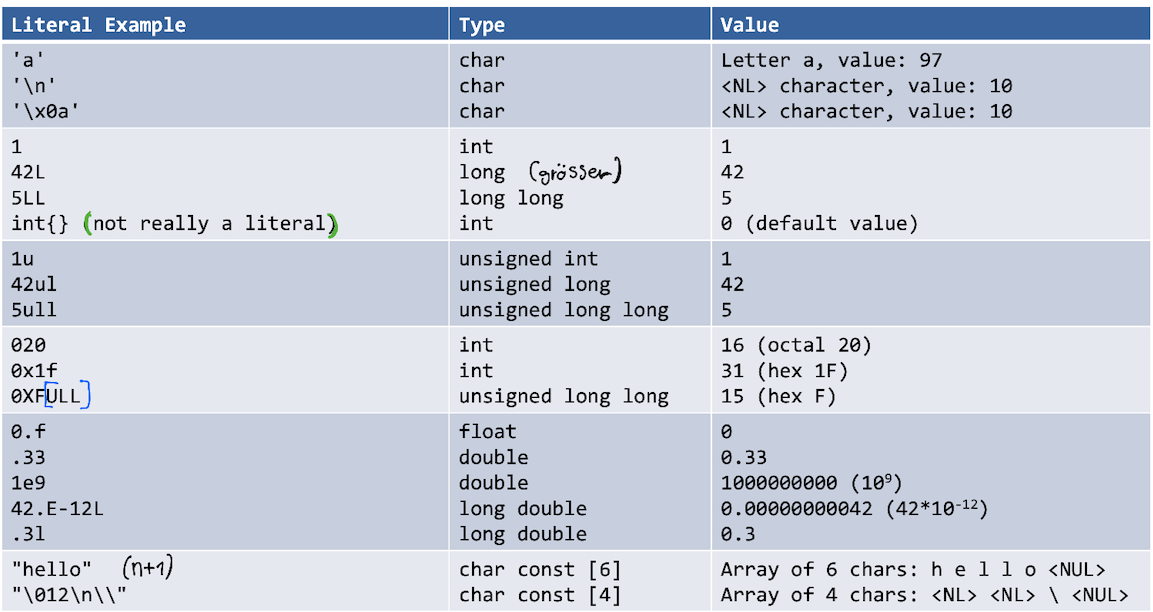
\includegraphics[width=0.75\linewidth]{images/literalexamples}

\begin{lstlisting}[language=C++]
(5 + 10 * 3 - 6 / 2) // precedence as in normal mathematics = 32
auto x = 3; / 3 // Fractions results of int operations always rundet down! 1
auto y = x%2 ? 1 : 0; // int to boolean conversion 0=false, all other are true. = 1
\end{lstlisting}

\subsection{Strings}
 std::string is C++'s type for representing sequences of char (which is often only 8 bit). This Strings are mutable in C++ in contrast to Java. Literals like "ab" are not of type std::string they consist of const chars in a null terminated array.
 
 To have a std::string we need to append an s. This requires using namespace std::literals;.
 
 \begin{lstlisting}[language=C++]
 void printName(std::string name) {
	using namespace std::literals;
	std::cout << "my name is: "s << name;
}	
\end{lstlisting}

\textbf{String Capabilites}\\
 You can iterate over the contents of a string.
\begin{lstlisting}[language=C++]
void toUpper(std::string & value) {
	for (char & c : value) {
		c = toupper(c); 
	}
}	
\end{lstlisting}

\subsection{Input and Output Streams}
Functions taking a stream object must take it as a reference, because they provide a side-effect to the stream (i.e., output characters).

\textbf{Simple I/O}
Stream objects provide C++'s I/O mechanism with the help of the pre-defined globals: std::cin std::cout. Should only be used in the main function! Streams have a state that denotes if I/O was successful or not.
\begin{itemize}
  \itemsep -0.5em 
  \item Only .good() streams actually do I/O
  \item You need to .clear() the state in case of an error
  \item Reading a std::string can not go wrong, unless the stream is already !good().
\end{itemize}

\textbf{Reading a std::strting Value }
\begin{lstlisting}[language=C++]
#include <iostream> 
#include <string>
	std::string inputName(std::istream & in) {
		std::string name{};
		in >> name;
		return name; 
}	
\end{lstlisting}
\textbf{Reading an int Value}
\begin{lstlisting}[language=C++]
int inputAge(std::istream& in) {
	int age{-1};
	if (in >> age) { // Boolean conversion
	return age; 
	} 
	return -1;
}
\end{lstlisting}
\textbf{Chaining Input Operations}
\begin{itemize}
  \itemsep -0.5em 
  \item Multiple subsequent reads are possible 
  \item If a previous read already failed, subsequent reads fail as well
\end{itemize}

\begin{lstlisting}[language=C++]
std::string readSymbols(std::istream& in) {
	char symbol{};
	int count{-1};
	if (in >> symbol >> count) {
		return std::string(count, symbol); 
	} 
	return "error";
}
\end{lstlisting}

\textbf{Stream States}\\
Formatted input on stream  is must check for is.fail() and is.bad(). If failed, is.clear() the stream and consume invalid input characters before continue.
\begin{center}
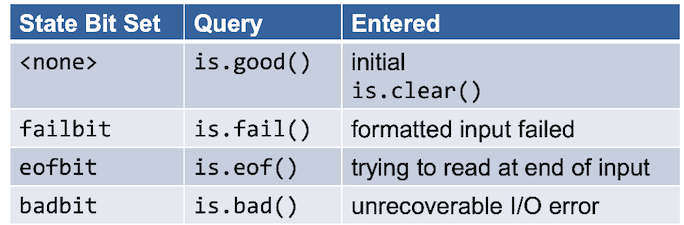
\includegraphics[width=0.75\linewidth]{images/streamstates}
\end{center}

\textbf{Headers}\\
As a general advise the most matching include should be used.
\begin{itemize}
  \itemsep -0.5em 
  \item $iosfwd$ contains only the declarations for std::ostream and std::istream. This is sufficient for function declarations.
  \item $istream$ and ostream contain the implementation of the corresponding stream, operators.
  \item $iostream$ contains all of the above and additionally std::cout, std::cin, std::cerr. This is only required in the source file containing the main() function, because only there the global standard IO variables shall be used

\end{itemize}
\break